
\chapter{Why}



In order to understand why this is happening, we examine a trace of the
experiment. We use schedviz~\cite{schedviz}, a tool that visualizes perf traces,
to examine the scheduling decisions Linux is making.

\begin{figure*}[t]
    \centering
    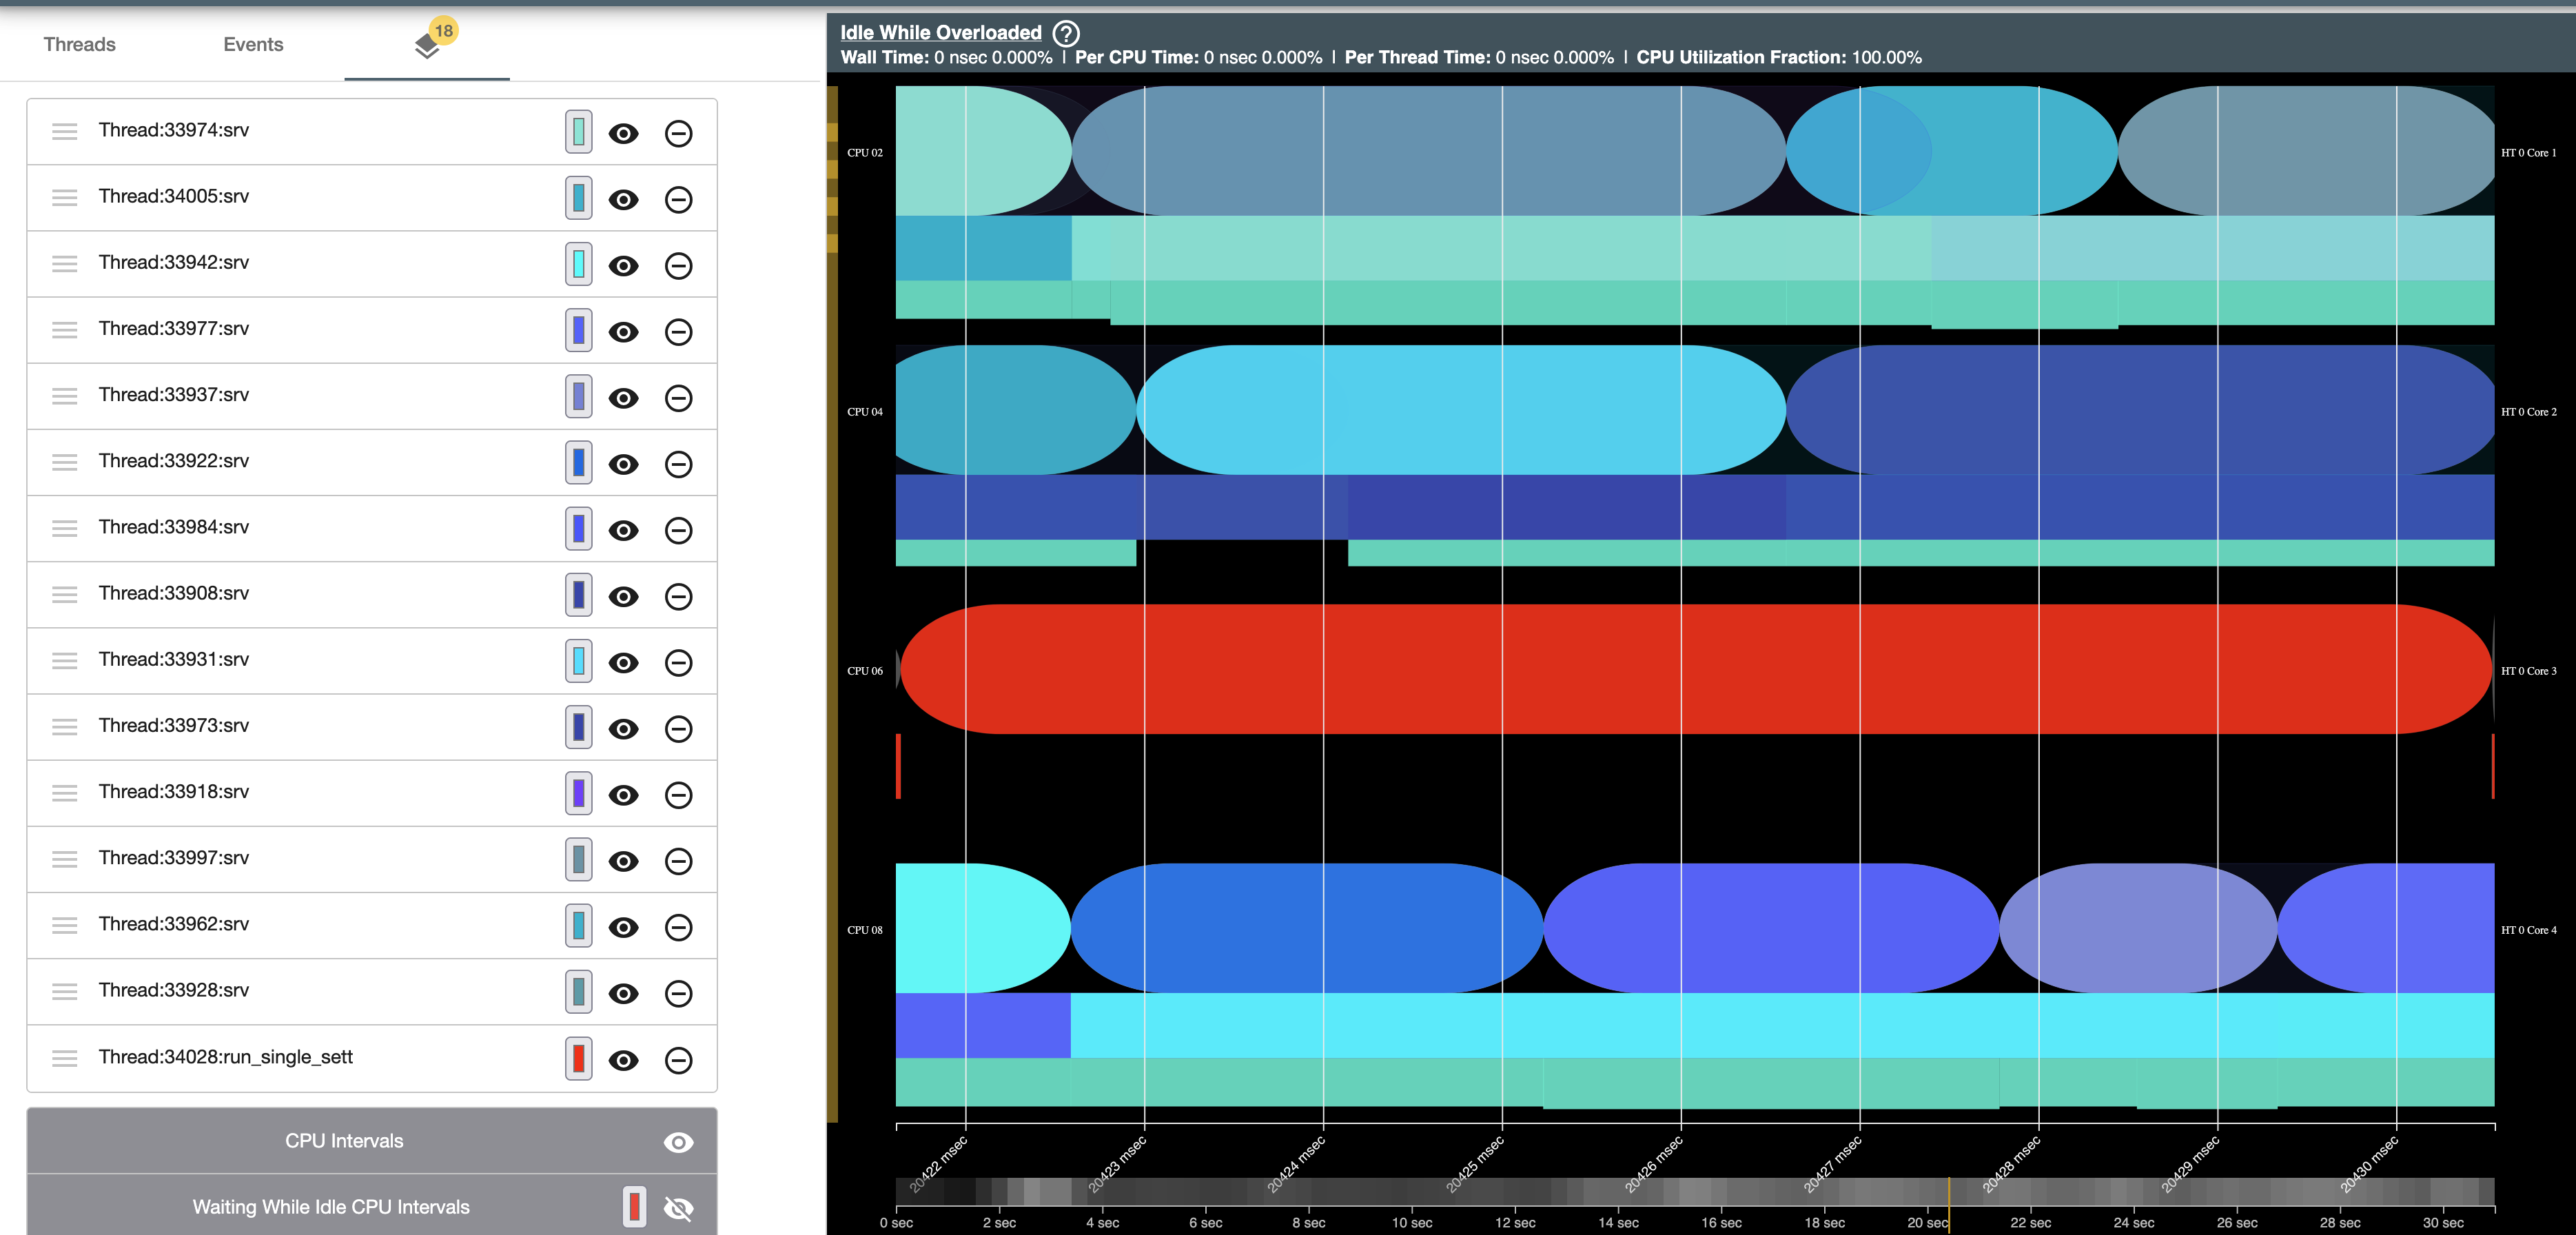
\includegraphics[width=\textwidth]{graphs/schedviz.png}
        \caption{Each thread is a different color. Circles represent which
    thread is running on that core, while rectangles underneath show waiting but
    runnable threads. Core numbers are 2,4,6,8 because this was run on a NUMA
    node so those are the cores that are closest to each other
    }\label{fig:schedviz}
\end{figure*}

In figure~\ref{fig:schedviz}, we look at a 10ms outtake from one of the runs,
that shows the problem occurring. The undesirable behavior we see here is that,
on core 6, the red process that is running the whole time is a BE process. All
the active server threads, shown in varying shades of blue, are on the other
cores, running and, more importantly, waiting.

The reason this happens is that Linux maintains a separate runqueue on each
core. This avoids the synchronization overheads of accessing global state for
every scheduling, but also means that the weight is only strictly enforced
within the individual runqueues, ie within each core. This leads to the depicted
failure mode, where an LC task is waiting on one core while another runs a BE
task.

% \hmng{should I also mention the giving at minimum 4ms? and how that can impact
%  tail latency}
